\documentclass{beamer}

\usepackage[T2A]{fontenc}
\usepackage[utf8]{inputenc}
\usepackage[english, russian]{babel}
\usepackage{paratype}
\usepackage{xcolor}
\usepackage{colortbl}
\usepackage{array}
\usepackage{tabularx}
\usepackage{booktabs}
\usepackage{mathrsfs,amsmath,amsthm,amssymb}

\usepackage{movie15}

\usepackage{tikz}
\usetikzlibrary{patterns}
\usepackage{pgfplots}
\pgfplotsset{compat=1.9}

\usepackage{mathtools}
\let\abs\relax
\DeclarePairedDelimiter\abs{\lvert}{\rvert}

\newcommand{\VovaSquare}[3]{\draw[thick] (#1-0.5*#3,#2-0.5*#3) --++ (#3,0) --++ (0,#3) --++ (-#3,0) -- cycle;}
\newcommand{\VovaCircle}[3]{\draw[thick] (#1,#2) circle (#3 cm);}
\newcommand{\VovaDot}[3]{\filldraw[thick] (#1,#2) circle (#3 cm);}
\newcommand{\VovaCross}[3]{\draw[thick] (#1,#2) --++ (#3,#3); \draw[thick] (#1,#2) --++ (-#3,#3); \draw[thick] (#1,#2) --++ (#3,-#3); \draw[thick] (#1,#2) --++ (-#3,-#3); }

\newcommand{\VovaSize}{0.3}

%\usetheme{Boadilla}
\usetheme{Pittsburgh}
\usecolortheme{seahorse}
%\usefonttheme[onlymath]{serif}
\usepackage{marvosym}
\usepackage{tikz}
\usetikzlibrary{graphs}
\usetikzlibrary{shapes, arrows}
\tikzstyle{decision} = [
                diamond,
                draw,
                fill = green!20,
                text width = 6em,
                text badly centered,
                node distance = 1cm,
                inner sep = 0pt
        ]
\tikzstyle{block} = [
                rectangle,
                draw,
                fill = blue!20,
                text width = 7em,
                text centered,
                rounded corners,
                minimum height = 3em
        ]
\tikzstyle{block0} = [
                rectangle,
                draw,
                fill = yellow!10,
                text width = 10em,
                rounded corners,
                minimum width = 10em
        ]
\tikzstyle{line} = [
                draw,
                -latex'
        ]

%Более крупный шрифт для подзаголовков титульного листа
\setbeamerfont{institute}{size=\normalsize}

\newcommand{\col}{\textcolor[rgb]{0.2,0.,0.55}}
\newtheorem{Th1}{Теорема 1}
\newtheorem{Th2}{Теорема 2}


%\AtBeginSection[]{
%  \begin{frame}
%  \vfill
%  \centering
%  \begin{beamercolorbox}[sep=8pt,center,shadow=true,rounded=true]{title}
%    \LARGE\insertsectionhead\par%
%  \end{beamercolorbox}
%  \vfill
%  \end{frame}
%}

\AtBeginSubsection[]{
  \begin{frame}
  \vfill
  \centering
  \begin{beamercolorbox}[sep=8pt,center,shadow=true,rounded=true]{title}
    \usebeamerfont{title}\insertsubsectionhead\par%
  \end{beamercolorbox}
  \vfill
  \end{frame}
}

\theoremstyle{plain}
%\newtheorem{d2}{Теорема}
\newcommand{\No}{ № }
\newcommand{\lambdahm}{\lambda_{h,m}}
\newcommand{\lambdahn}{\lambda_{h,n}}
\newcommand{\lambdahmn}{\lambda^{h,mn}}
\def\cfrac#1#2{\displaystyle{\frac{#1}{#2}}}

\begin{document}

\title{{О  решении линеаризованной системы двумерной динамики вязкого газа}}
\author[%
	Назаров В.\ С.
]{%
\begin{center}
	Выполнил аспирант \\
	{\bfseries Назаров Владимир Сергеевич }
	\\ \vspace*{0.5cm}
	%\begin{flushright}
	{\scriptsize
	Научный руководитель: \\
    д.\,ф.-м.\,н., 
	профессор {\bfseries Корнев Андрей Алексеевич}}
	%\end{flushright}
	\\ \vspace*{0.4cm}
	{\scriptsize 
	Современные проблемы математики и ее приложений}
	\\ \vspace*{0.2cm}
{\tiny Международная (53-я Всероссийская) молодежная школа-конференция \\ 31 января -- 4 февраля 2022 г., г. Екатеринбург}
	\end{center}
}
\date{
\scriptsize{СоПроМат "--- 2022}
}


	\begin{frame}
		\begin{center}
			\footnotesize{МГУ имени М. В. Ломоносова}\\
			\footnotesize{Механико-математический факультет} \\
			\footnotesize{Кафедра вычислительной математики}\\\vspace{8pt}
		\end{center}
		\titlepage
	\end{frame}


	
	\section{Постановка задачи}


	
	\begin{frame}[shrink=0]{Постановка задачи}
	
Система уравнений 
$$
\begin{cases}
&\cfrac{\partial \rho}{\partial t} + \cfrac{\partial \rho u}{\partial x}+ \cfrac{\partial \rho v}{\partial y} = 0, \\
&\cfrac{\partial \rho u}{\partial t} + \cfrac{\partial \rho u^2}{\partial x} + \cfrac{\partial \rho u v}{\partial y} 
	+ \cfrac{\partial p}{\partial x} 
	= \mu \Big(\cfrac{4}{3}\cfrac{\partial^2 u}{\partial x^2} + \cfrac{\partial^2 u}{\partial y^2}
	+  \cfrac{1}{3}\cfrac{\partial^2 v}{\partial x\partial y} \Big) + \rho f_1, \\
&\cfrac{\partial \rho v}{\partial t} + \cfrac{\partial \rho u v}{\partial x} + \cfrac{\partial \rho v^2}{\partial y}
	+ \cfrac{\partial p}{\partial y} 
	= \mu \Big(\cfrac{1}{3}\cfrac{\partial^2 u}{\partial x\partial y} + \cfrac{\partial^2 v}{\partial x^2}
	+  \cfrac{4}{3}\cfrac{\partial^2 v}{\partial^2 y} \Big) + \rho f_2,
\end{cases}
\eqno(1)
$$
описывает  нестационарное двумерное движение вязкого баротропного газа.
Здесь $\mu$ - коэффициент вязкости газа (известная неотрицательная константа), 
$p=p(\rho)$ - давление газа (в работе рассматривается случай  $p=C_\rho \rho$), 
$(f_1,f_2)^T$ - вектор внешних сил.
Искомые функции, т.е.  плотность $\rho$, скорость $u$ вдоль оси $OX$,  скорость $v$ вдоль оси $OY$   являются функциями переменных Эйлера ${(t,\,\, x,\,\, y) \in [0,\,\, T] \times \Omega}$.

	\end{frame}
	
	\begin{frame}[shrink=10]{Линеаризация}
Построим линеаризацию в окрестности 
стационарного состояния 
$(\rho_{st}, u_{st},v_{st}) = (\rho_0, 0, 0)$ при нулевой правой части и запишем её 
с сохранением исходных обозначений. Отметим также, что $C_{\rho}=p'(\rho_{st})$.
Получим следующую систему: 
$$
\begin{cases}
&\cfrac{\partial \rho}{\partial t} 
+ \rho_0\cfrac{\partial  u }{\partial x} 
+ \rho_0 \cfrac{\partial v }{\partial y} = 0, \\
&\rho_0 \cfrac{\partial u}{\partial t} 
+ C_{\rho} \cfrac{\partial \rho}{\partial x} 
= \mu \Big( \cfrac{4}{3}\cfrac{\partial^2  u}{\partial x^2} + \cfrac{\partial^2  u}{\partial y^2}
	+  \cfrac{1}{3}\cfrac{\partial^2  v}{\partial x\partial y} \Big) , \\
&\rho_0 \cfrac{\partial  v}{\partial t} 
+ C_{\rho} \cfrac{\partial \rho}{\partial y} 
= \mu \Big( \cfrac{4}{3}\cfrac{\partial^2 v}{\partial y^2} + \cfrac{\partial^2 v}{\partial x^2}
	+  \cfrac{1}{3}\cfrac{\partial^2  u}{\partial x\partial y} \Big) \end{cases}
\eqno(2)
$$
относительно вектор-функции $\mathbf{w}(t,x,y) = (\rho,  u, v)^T$, удовлетворяющую
 начальным и периодически продолжаемым граничными условиям следующего вида:
$$
\begin{array}{cc}
&(\rho, u, v)|_{t=0} = (\rho^0, u^0, v^0),\,\, (x,\,y) \in \Omega = [0; 2\pi] \times [0; 2\pi]; \notag \\
&u(t,\, x,\, y)|_{x=0, 2\pi} = 0,\,\,  u_y(t,\, x,\, y)|_{y =0, 2\pi} = 0,  \\
&v_x(t,\, x,\, y)|_{x = 0, 2\pi} = 0,\,\,  v(t,\, x,\, y)|_{y =0, 2\pi} = 0,\,\, t \in [0;\, T]. \notag
\end{array}
\eqno(3)
$$

	\end{frame}	
	
	\section{Обзор результатов}

	\begin{frame}[shrink=40]{Теоретические результаты}
	
\begin{Th1}
Пусть начальные функции 
 $\rho^0\in W^1_2(\Omega)$, 
$u^0,v^0  \in W_2^{2}(\Omega)$   имеют следующий вид: \\
\noindent $
\rho^0 (x,\, y) = 
\sum\limits_{\substack{n=0 \\
m=0}}^{\infty} P_{mn}^0 \cos \frac{mx}{2} \cos \frac{ny}{2}, \;
u^0 ( x,\, y) = \sum \limits_{\substack{m=1 \\
n=0}}^{\infty} C_{mn}^0 \sin \frac{mx}{2} \cos \frac{ny}{2},  \;
 v^0 (x,\, y) = \sum  \limits_{\substack{m=0 \\
n=1}}^{\infty} D_{mn}^0 \cos \frac{mx}{2} \sin \frac{ny}{2}. 
$

Пусть $\forall m,n \ge 0$ выполняется
$\frac{9 C_\rho \rho_0^2}{\mu^2} \ne (m^2+n^2)$.
Тогда решение  задачи (2), (3) можно представить в следующей форме:
$$
\mathbf{w} (t,\, x,\, y) = 
\begin{pmatrix}
\rho(t,\, x,\, y) \\
u(t,\, x,\, y) \\
v(t,\, x,\, y) 
\end{pmatrix} = 
K_0 \mathbf{\Psi}_0 + \sum \limits_{\substack{m,n=0 \\
m+n>0}}^{\infty} 
\sum \limits_{l=1}^3\Big(
K_l^{nm} \exp (\lambda_l^{nm} t) \mathbf{\Psi}_l^{nm}
\Big), 
\eqno(4)
$$
$$\mbox{ где  } \lambda^{mn}_1 = -\frac{\mu (m^2 + n^2)}{4 \rho_0}, \quad
\lambda^{mn}_{2,3} = \frac{2}{3} \lambda^{mn}_1  \pm  
\sqrt{  \left(\frac{2}{3} \lambda^{mn}_1\right)^2   - \frac{C_\rho(m^2+n^2)}{4} },
$$

$$
\mathbf{\Psi}_0 = 
\begin{pmatrix}
1 \\ 0 \\ 0
\end{pmatrix}
\mbox{, }
\mathbf{\Psi}_{l}^{mn} = 
\begin{pmatrix}
\xi_{{l}_1}^{mn} \cos \frac{mx}{2} \cos \frac{ny}{2}\\ 
\xi_{{l}_2}^{mn} \sin \frac{mx}{2} \cos \frac{ny}{2}\\
\xi_{{l}_3}^{mn} \cos \frac{mx}{2} \sin \frac{ny}{2}
\end{pmatrix},\quad l=1,2,3;
$$
$$
\xi_l^{mn} = 
\Big(
\xi_{l_1}^{mn}, \xi_{l_2}^{mn}, \xi_{l_3}^{mn}
\Big)^T, \quad
\xi_1^{mn} =  (0, n, -m)^T, \quad
\xi_{2,3}^{mn} = (\lambda_{3,2}, - \frac{m C_\rho}{2 \rho_0} , -
\frac{n C_\rho}{2 \rho_0} )^T.
$$
Здесь $K_0=P^0_{00}$ , 
а коэффициенты $(K_1^{mn},K_2^{mn},K_3^{mn})^T$,  $m+n>0$,
однозначно восстанавливаются из начальных условий
$\sum\limits_{l=1}^3 K_l^{nm} \xi_l^{mn} = (P^0_{mn}, C^0_{mn}, D^0_{mn})^T$.
\end{Th1}
\end{frame}

\begin{frame}
\begin{Th2}  В условиях теоремы 1 верна оценка:
$
\displaystyle \| \mathbf{w}(t) - \mathbf{w}_{st} \|_{L_2(\Omega)} \leqslant \mathcal{A} e^{ \delta t} \| \mathbf{w}(0) -\mathbf{w}_{st} \|_{L_2(\Omega)}, \;
$
где 
 $\delta = \max \{ -\frac{\mu}{6\rho_0},\,\, 
 - \frac{\mu k_1^2 }{6 \rho_0}
 + \frac{\mu k_1^2}{6 \rho_0} \sqrt{ 1    - \frac{9 C_\rho \rho_0^2 }{\mu^2 k_1^2} },
 - \cfrac{3 C_{{\rho}} {{\rho}_0}}{4 \mu} \}, \;
 \mbox{ при }   k_1 = \min (k) :  k^2 \ge  \frac{9 C_\rho \rho_0^2 }{\mu^2 }.
 $

Здесь 
$
\mathbf{w}_{st} = (p_{st},\, u_{st},\, v_{st}),\, 
p_{st}=\cfrac{1}{4\pi^2} \int \limits_0^{2\pi} \int \limits_0^{2\pi} p^0 dxdy = K_0, 
\; u_{st}=0,\, v_{st}=0$.
\end{Th2}
	\end{frame}	
	
\begin{frame}[shrink=0]{Конечно--разностная аппроксимация}

Для решения исходной задачи будем использовать   полностью неявную схему
$$
\begin{cases}
&P_t + {\rho}_0 \hat U_x  + {\rho}_0 \hat V_y  = 0,  \\
&{\rho}_0 U_t + C_{\rho}\hat P_{\bar x} = \mu \Big( \frac{4}{3} \hat U_{x\bar x} + \hat U_{y\bar y} + \frac{1}{3} \hat V_{x y}
\Big), \\
&{\rho}_0 V_t + C_{\rho}\hat P_{\bar y} = \mu \Big( 
\frac{4}{3} \hat V_{y\bar y} + \hat V_{x\bar x} + \frac{1}{3} \hat U_{x y}\Big),
\end{cases}
\eqno(5)
$$
построенную на смещенных сетках В.И. Лебедева:
	\begin{figure}[h!]
\begin{minipage}[h]{0.6\linewidth}
\begin{tikzpicture}
		\draw[step=1.2cm,dotted] (0,0) grid (5,4);
		\foreach \x in {0,...,3}{
			\foreach \y in {0,...,3}{
				\VovaSquare{1.2*\x+0.6}{1.2*\y}{\VovaSize}
			}
		}
		\foreach \x in {0,...,4}{
			\foreach \y in {0,...,2}{
				\VovaCircle{1.2*\x}{1.2*\y+0.6}{0.5*\VovaSize}
			}
		}
		\foreach \x in {0,...,3}{
			\foreach \y in {0,...,2}{
				\VovaCross{1.2*\x+0.6}{1.2*\y+0.6}{0.5*\VovaSize}
			}
		}
		\foreach \x in {0,...,4}{
			\foreach \y in {0,...,3}{
				\VovaDot{1.2*\x}{1.2*\y}{0.1}
			}
		}
		% Поясняющий текст
		\VovaSquare{8}{1}{\VovaSize} ; \draw (8,1) node[right]
{\mbox{  }  --  \bfseries V};
		\VovaCircle{8}{2}{0.5*\VovaSize}; \draw (8,2) node[right]
{\mbox{  }  --  \bfseries U};
		\VovaCross{8}{3}{0.5*\VovaSize}; \draw (8,3) node[right]
{\mbox{  }  --  \bfseries P};
		
\end{tikzpicture}	
\end{minipage}
\end{figure}

\end{frame}


\begin{frame}[shrink=40]{Численные результаты}

Общая картина динамики 
выхода на стационар решений дифференциальных задач
для начальных возмущений типа  скачок скорости
$$
  p_1^0(x,y) = 1,\quad  0 \le x,y\le 2\pi,
  \quad
  u_1^0(x,y) = v_1^0(x,y) =
  \begin{cases}
    1 \quad \  4\pi/5 \le x,y \le  6\pi / 5, \\
    0 \quad \text{ иначе};
  \end{cases}
$$
и скачок плотности
$$
 p_2^0(x,y) = 
  \begin{cases}
    2 \quad \  4\pi/5 \le x,y \le 6\pi / 5, \\
    1 \quad \text{ иначе},
  \end{cases}
  \quad
  u_2^0(x,y) = v_2^0(x,y) =0, \quad  0 \le x,y\le 2\pi.
$$

\begin{tabular}{cc}
 \begin{tabular}{c}
%D:\cygwin64\home\kornev\2020\2020_Num\NumSDS\task\20-Gas2d\Numres\UVPJumpSqPi\
 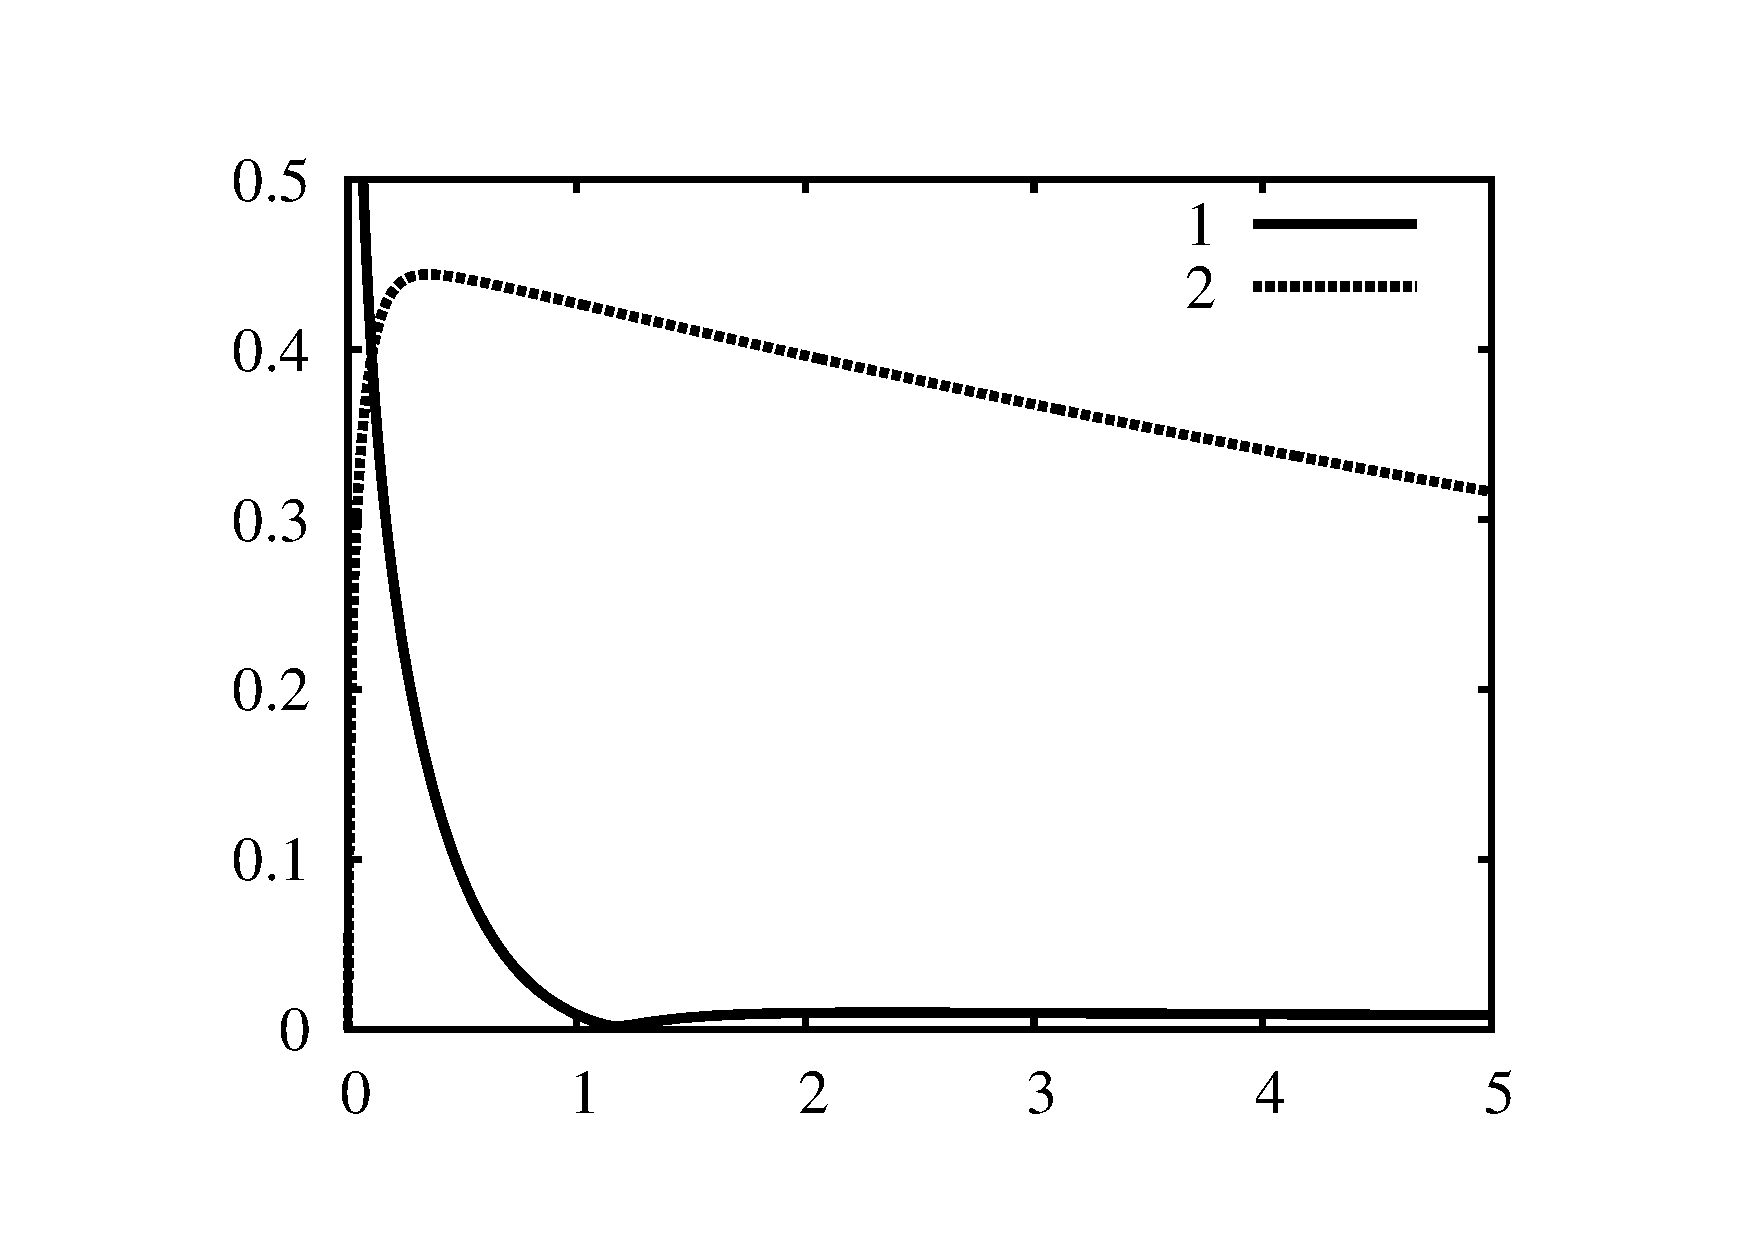
\includegraphics[width=9cm]{./Picts/JumpDist.pdf}\\
  Рис. 1. Графики функций 
  $\|(u_{i}(t),v_i (t)\|_{L_2(\Omega)}$ \\
  при $\mu = C_{\rho} = 1, \rho_0 = 0,1$. \\
   {\it i=1}~--- скачок скорости; {\it i=2}~---  скачок плотности.
\end{tabular}
&
 \begin{tabular}{c}
\hfill Скачок плотности. Табл. 1. \\
 \begin{tabular}{|c|c|c|c|}
    \hline
    $K^{mn}_2$     & n=0    & n=1    & n=2  \\
    \hline
    m=0                  & 0.08206  &  0.01525  & -0.13711 \\
    \hline
    m=1                  & -0.01275 & -0.00194  & 0.01525 \\
    \hline
    m=2                   &  0.00000 & -0.01275  & 0.08206 \\
    \hline
  \end{tabular} \\
  \\
\hfill Скачок скорости. Табл. 2. \\
  \begin{tabular}{|c|c|c|c|}
    \hline
    $K^{mn}_2$     & n=0    & n=1    & n=2  \\
    \hline
    m=0                  & 0.00014 & -0.00052 & -0.00023  \\
    \hline
    m=1                  & 0.00230 &  0.00034 & -0.00052  \\
    \hline
    m=2                  &  0.00000 &  0.00230  & 0.00014  \\
    \hline
  \end{tabular}
\end{tabular}

\end{tabular}

Наличие аналитических формул для решения позволяет объяснить данный  эффект.
В Табл.  1,2  приведены  приближенные значения старших коэффициентов 
$K^{mn}_2$, $m,n=0,1,2$,
при разложении указанных начальных возмущений.

\end{frame}

\section{Спасибо за внимание}

\begin{frame}
\begin{center}
	\Huge{\color{blue}{Спасибо за внимание!}}
	\end{center}
\end{frame}

\end{document}
